\justifying
\section{Introduction}
According to Hegel's dialectic process (\textit{Entwicklung}; development), the progress and the creation of knowledge originates from clashing of opposing sides and is constituted by a triad.\cite{hegel1807phenomenology} First (\textit{An-sich}; per-se), we discover the definition of a concept, then a second concept is introduced (\textit{Anderssein}; be different), which abolishes or cancels the first. As a result of this opposition, during the last step of the process (\textit{An-und-f{\"u}r-sich}; on-and-for-itself) a third new concept is introduced, which is higher and truer compared to the original. Fitche described this triad in what is most commonly known as the thesis-antithesis-synthesis. The dialectic process can also be observed in the world surrounding us and in the progress of science.\cite{fichte1993fichte}\\
For instance, social media is an interesting example of synthetic evolution. On the one hand, simple social interaction can be described as a sort of physical instinct movement with a specific individual purpose. On the other hand, mass media can be described as the electronic transmission of information invisible to human senses with primary marketing purposes. From the opposition between these two spheres, social media arises in which the interaction has lost the animal and physical-like interaction for a possibly greater and more expansive interaction (\textit{i.e.}, one-on-one versus one-on-many). An evident example in science is the advance in robotics with the creation of androids, generated from the synthesis of humans and machine. Another example found in science is the description of fluid motion. In general, we can describe the behavior of a system from a macro and continuum (Navier-Stokes) perspective; on the other hand, the same system could also be described by a particle-particle (molecular) interaction perspective given extreme computational power. Nowadays, there are available methods that synthesize these two perspectives by treating the system with novel intermediate mesoscale concepts such as Lattice-Boltzmann, which allows a mesoscale description of the system useful at length scale for which the continuum body assumption breaks down, but the dimension of the system is too large to be considered particle-particle interaction.\cite{amadei2017role}\\
Synthetic advances via the Hegelian process can also be observed in the study of water engineering. For instance, desalination was first widely practiced utilizing thermal processes such as distillation. Today, membrane desalination technology has become predominant in practice separating water from ions through reverse osmosis (RO). The synthesis of thermal and membrane technology has, in turn, sparked a new line of research in membrane distillation, highlighting the importance of the synthetic approach.\cite{bhadra2016desalination} In the sub-topic of water treatment membranes materials, two opposing research fields can be distinguished: ceramic versus polymeric membranes. On the one hand, ceramic membranes excel in thermal and chemical stability and the simplicity of their cleaning process. On the other hand, polymeric membranes feature thinness, cost-effectiveness, and  ease of property manipulation, which allows them to excel in industrial and municipal applications such as ultra-/nano-filtration (UF/NF).\cite{baker2004overview}\\
A chemically and thermally resistant membrane resilient to harsh cleaning (typical of ceramic membranes) and able to operate in the nanofiltration regime (dominated by polymer membranes) has potential for advanced wastewater treatment (AWWT) applications. AWWT aims to convert wastewater into water that can be reused, depending on its quality, for other purposes such as urban, agricultural, environmental, and potable uses. Although AWWT varies depending on feed quality and on the standard effluent requirements, membranes processes are generally used to remove ions and organic molecules to meet the strict environmental standards. Nowadays, membrane processes in AWWT are dominated by polyamide polymeric membranes, which are subject to fouling and cleaning issues due to their poor chemical resistance.\cite{safarpour2015thin} Membrane fouling leads to increased treatment plant operations and maintenance (O\&M) cost due to several reasons such as cleaning chemical cost and increased plant downtime. For instance, a two-fold more expensive chlorine-resistant nanofiltration membrane will lead to savings in the overall plant O\&M due to the reduction of chemicals use and downtime.\cite{dave2017six} Similarly, other studies estimated that at least 50\% of O\&M is dominated by membrane cleaning and replacement.\\
Previous studies have investigated using a protective layer to enhance the selectivity or the chemical stability of the membranes. For example, GO embedded in RO membranes drastically improved the chlorine resistance due to the prevention of polyamide chlorination.\cite{chae2015graphene} However, the chemical resistance was limited to the selective layer, as the polymer-based substrate was subject to degradation when oxidizing agents permeate the membranes.\cite{goh2015all,amadei2016increase} Moreover, polymer-based membranes will also limit the membrane operating temperature as well as permeating fluid properties.\\
Motivated by the aim to develop cost-effective AWWT solutions, we hypothesized that a Fully Carbon Membrane (FCM) operating in the NF regime could be manufactured with the exclusive use of fully carbon nanomaterials with no polymers, \textit{i.e.}, the elemental composition of all materials is $>75$\% carbon and the monomer repeating units of a polymer have been replaced with elemental carbon architectures. To our knowledge, this is the first study to manufacture a filtration FCM in all its components: from the mechanical substrate to the selective layer.\cite{goh2015all}\\
In this study, a FCM was manufactured via a 3D printed custom-made vacuum filtration system with the use of carbon fiber (CF), carbon nanotubes (CNT), and GO. The potential of the FCM for AWWT is focused on two main performance measures: i) the capability of the membranes to reject ions in a cross-flow apparatus (typical in municipal applications) before and after harsh cleaning processes; and ii) the chemical and thermal resistance of the membranes challenged by permeation of oxidizing agents and annealing cycles. The FCMs were characterized via a combination of surface characterization tools (scanning electron microscopy and X-ray photoelectron spectroscopy), capillary flow porometry, thermogravimetric analysis, and ion rejection evaluation. 


\section{Methods}

\subsection{Chemicals and Materials}
The \textit{Spectracarb 2050-1050 GDL} CF paper was purchased from \textit{Engineering Fiber Technology}. C-grade multiwalled nanotubes (CNTs) with $>95$\% purity were purchased from \textit{NanoTechLabs} (Yadkinville, NC). Graphene oxide (GO) aqueous solutions ($\approx4$ mg/mL) were purchased from \textit{Graphenea} (Cambridge, MA). Sodium sulfate (NaSO4, $\approx99$\%), sodium chloride (NaCl, $\approx97$\%), and sodium hydroxide (NaOH, $\approx97$\%) were purchased from \textit{Sigma-Aldrich}, sodium hypochlorite (NaClO, 8\%) and isopropyl alcohol (IPA, 99\%) were purchased from \textit{VWR chemicals}, and 5 wt\%  Nafion solution was purchased from \textit{Fuel Cell Earth} (Woburn, MA).

\subsection{Fully Carbon Membrane Fabrication}
A flowchart in Fig.~\ref{figS1_AppD} in the Appendix D summarizes the overall fabrication process. First, a CNT solution was prepared by mixing 30 mg of CNT with 60 mL of IPA and 0.2 mL of Nafion solution (5 wt\%), then dispersed by probe-sonication (Sonifier S-450D with high gain horn; \textit{Branson Ultrasonics Corp.}) at 50\% of the maximum amplitude (100 W) for 3 min, and subsequently, bath sonicated for 4 min in a \textit{Branson} sonicator ($V=1.9$ L, maximal power $=80$ W, and $f=20$ kHz). The obtained CNT solution was vacuum filtered onto a CF paper (1\textsuperscript{st} layer, substrate of the FCM) using a custom 3D printed filtration system (see Fig.~\ref{figS2_AppD} in the Appendix D). Another solution containing GO and CNT was prepared in the same manner as the first CNT solution but also included 0.15 mL of GO solution ($\approx4$ mg/mL) added prior to the bath sonication step. This GO-CNT solution was then vacuum filtrated onto the CF-CNT composite substrate, constituting a transition layer between the intermediate CNT support layer (2\textsuperscript{nd} layer) and the final GO selective layer (3\textsuperscript{rd} layer). Then, a 0.2 mL GO solution ($\approx4$ mg/mL) was diluted with 80 mL of DI water and bath sonicated for 1 min. The final GO solution was then filtered onto the GO-CNT transition layer, constituting the selective layer of the FCM. Finally, the FCM was thermally reduced at 150 \textdegree C for 20 min in an inert atmosphere (\textit{i.e.}, N\textsubscript{2}) with the use of a \textit{Thermolyne 21100} tube furnace, in order to increase membrane stability. Once the FCM was prepared, it was cut with a razor blade in a rectangular shape (8 x 4 cm\textsuperscript{2}) and placed into the filtration device for testing. FCM were initially tested for integrity by permeating through DI at 5 bar of applied pressure and only those passing the test (\textit{i.e.}, permeability $<30$ LMH-bar (\textit{i.e.}, L m\textsuperscript{-2}h\textsuperscript{-1}bar\textsuperscript{-1}) indicating overall structural integrity) were used in subsequent experiments.


\subsection{Fully Carbon Membrane Characterization}
\textbf{Scanning electron microscopy (SEM):} The morphology and structure of the FCMs were characterized using a \textit{Zeiss ULTRA} Field Emission Scanning Electron Microscope with an In-lens secondary electron detector. The working distance was $3-4$ mm, and the acceleration voltage was 5 kV. The statistical SEM image analysis of the FCM layers was completed using \textit{ImageJ} software.\\
\textbf{X-Ray photoelectron spectroscopy (XPS):} FCM surface chemistry was analyzed by a \textit{Thermo Scientific K-Alpha} XPS instrument (ESCA) with X-rays generated by a 12 kV electron beam with a spot size of 400 $\mu$m. The O/C ratio and peak deconvolution were quantified by \textit{Thermo Scientific Avantage} software, and then converted to mass ratio by using C and O atomic weights. The XPS instrumental error for atomic composition is $\pm$1\%, and the accuracy of the C1s peak fitting is $\pm$2\%.\\
\textbf{Thermogravimetric analysis (TGA):} The FCM thermal stability was evaluated with a \textit{Discovery TGA}. The samples were cut into 5 x 5 mm\textsuperscript{2} pieces for a total weight of $\approx5$ mg. The target temperature was set to 500 \textdegree C with a 10 \textdegree C/min heating rate under air flow (25 mL/min). The mass change over time was monitored and quantified with \textit{Trios} software.
\subsection{Permeability and Rejection Test}
The FCMs were tested using a multi-cell cross-flow apparatus (see Fig.~\ref{figS3_AppD} in the Appendix D). The cross-flow apparatus allows the simultaneous evaluation of nine membranes at a pressure ranging from 4 to 10 bar. The effective filtration area for each membrane is 7 x 3 cm\textsuperscript{2}.  The pure water permeability, expressed in LMH-bar, was evaluated by monitoring the permeate volume with a \textit{Sartorious} laboratory balance every 30 or 60 min.
The permeate was collected in vials and the conductivity rejection ($R$)was calculated with eqn~(\ref{eqn1_pap5}): 
\begin{equation}
  R ={\Big(1- \dfrac{C_{p}}{C_{f}}\Big)*100}
 \label{eqn1_pap5}
\end{equation}

where $C\textsubscript{p}$ and $C\textsubscript{f}$ are the conductivity of the permeate and the feed, respectively. The conductivity rejection tests were carried out with a 1 mM NaCl and 1 mM NaSO\textsubscript{4} aqueous solution. The conductivity rejection was determined with a \textit{ThermoFisher Scientific} conductivity probe. 
The individual ion rejection ($R_{ion}$) was calculated with equation similar to eqn~(\ref{eqn1_pap5}): 
\begin{equation}
  R_{ion} ={\Big(1- \dfrac{C_{ion,p}}{C_{ion,pf}}\Big)*100}
 \label{eqn2_pap5}
\end{equation}

where $C\textsubscript{ion,p}$ and $C\textsubscript{ion,f}$ are the specific ion concentration of the permeate and the feed, respectively. The anion (Cl\textsuperscript{-} and SO\textsubscript{4}\textsuperscript{2-}) concentrations were measured with a \textit{Dionex ICS-3000} Ion Chromatograph (\textit{Dionex Corporation}, Sunnyvale, CA) consisting of a SP single pump, DC detector, \textit{AS40} autosampler, and a \textit{Chromeleon 6.8} software. cl\textsuperscript{-} and SO\textsubscript{4}\textsuperscript{2-} were separated from other anions using a \textit{Dionex IonPac AS25} analytical column (4.0 x 250 mm\textsuperscript{2}) and a \textit{Dionex IonPac AS25} guard column (4.0 x 50 mm\textsuperscript{2}) with anion self-regenerating suppressor (ERS 500) in recycle mode. Mobile phase (21 mM NaOH) was prepared using a 50\% (w/w) sodium hydroxide aqueous solution and deionized water (18.2 M$\Omega$-cm). The isocratic eluent flow rate was 1 mL/min for 6 min with an injection volume of 50 $\mu$L and a column temperature of 30 \textdegree C. Quantification of individual ions was done using a five-point linear calibration curve over the range of $5-100$ mg/L. All samples were diluted before injection and blanks were included in each run. Standard additions were used to confirm the retention time of each anion.
Theoretical ion rejection can also be calculated using eqn~(\ref{eqn3_pap5}):\cite{Davisbook}
\begin{equation}
  R_{ion} ={\Big(1- 2\Big(1-\dfrac{d_{ion}}{d_{pore}}\Big)^2+\Big(1-\dfrac{d_{ion}}{d_{pore}}\Big)^4 \Big)*100}
 \label{eqn3_pap5}
\end{equation}


where $d\textsubscript{ion}$ and $d\textsubscript{pore}$ are the diameter of the hydrated ions and of the membrane pores, respectively.
The wet flow curves of the membranes were calculated by the capillary flow porometry (CFP) method using a gas-liquid displacement Porometer (\textit{POROLUX\textsuperscript{TM} 100}, Porometer). CFP is based on the displacement of a wetting liquid inside a porous network by means of an inert gas flow. In this study, POREFIL\textsuperscript{\tiny\textregistered} (Porometer, surface tension $\gamma = 16$ dyne/cm) was used as the wetting liquid agent, compressed air was used as the inert gas, and the pressure scan method was applied within a pressure range of $0-5.5$ bar at room temperature ($\approx23$ \textdegree C). The membranes were first wetted by the \textit{POREFIL\textsuperscript{\tiny\textregistered}} and the gas permeation flow was measured by increasing the transmembrane pressure at a rate of 0.0125 bar/s to obtain the wet curve. The diameter of all the samples was 18.5 mm. At least three different samples for each membrane were evaluated to obtain the final reported wet flow curve.

\subsection{Fully Carbon Membrane Stability}
The chemical stability of the FCM was evaluated by comparing the membrane performance (rejection and permeability) before and after 9 hr of NaClO filtration at 1000 ppm and 5 bar of applied pressure. Moreover, the surface chemistry of the FCM exposed to chlorination was compared to that of the control ones (exposed to DI). In terms of thermal stability, the surface chemistry of membranes exposed to multiple annealing cycles (up to four) at 150 \textdegree C in air was compared to the chemistry of membranes exposed to a single annealing cycle to evaluate any thermal modifications of the surface. Moreover, TGA analysis were also performed here to observe the loss in mass of FCMs exposed to annealing cycles in air.

\section{Results and discussion}
\subsection{Fully Carbon Membrane Characterization}

A FCM is characterized by a hierarchical structure composed of three layers: a CF layer, a CNT layer, and a GO layer as displayed in Fig.~\ref{Fig1_pap5}. More details about these three layers can also be found in the SEM images displayed in Fig.~\ref{figS4_AppD}. The quantitative morphology dimensions of these carbon nanostructures, summarized in Table~\ref{tbl1_pap5}, were determined via statistical analysis (see Fig.~\ref{figS5_AppD} for more detail) of the SEM images in Fig.~\ref{figS4_AppD} in the Appendix D.

\begin{figure}%[h!]
  \centering
  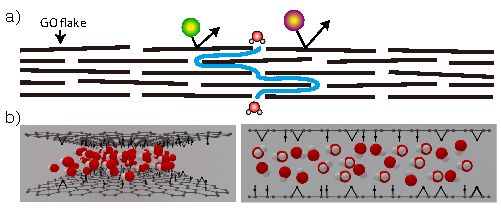
\includegraphics[width=2.8in]{paper5/Fig1.pdf}
  \caption{\textbf{FCMs advantages and hierarchical structure.} \textbf{(a)} Advantages of FCMs derived from the Hegelian approach. \textbf{(b)} Schematic of the hierarchical structure of a FCM composed of three layers (GO, CNT and CF). \textbf{(c)} SEM images of a FCM: top image is a cross-section of a FCM, middle image is a zoom-in of the cross-section (the extension of the CNT and GO layers are indicated with arrows) and bottom image is an aerial view of the FCM in which the three carbon architectures (CF, CNT, and GO) are visible.}
  \label{Fig1_pap5}
\end{figure}


\begin{table}
 \begin{center}
 \caption{\textbf{Specifications of the FCM hierarchical structure.}}
  \label{tbl1_pap5}
  \begin{tabular}{cccc}
        \hline
        Layer & Material & Dimension & Elemental composition\\
         &  & (SEM) & (XPS)\\
        \hline
        1\textsuperscript{st} & Carbon Fiber  & CF Diameter: $6.8\pm0.5$ $\mu$m & C: $95.1\pm1.0$ \%\\
        & (CF) & Thickness: $160\pm10$ $\mu$m & O: $4.5\pm1.0$ \%\\
        &  & Pore Size: $41\pm5$ $\mu$m\textsuperscript{*} & \\
        2\textsuperscript{nd} & Carbon Nanotubes  & CNT Diameter: $16.5\pm1.3$ nm & C: $78\pm1.0$ \%\\
         &(CNT)-Nafion  & Thickness: $\approx10$ $\mu$m & F: $19.1\pm1.0$ \%\\
        &(includes intermediate & Pore Size: $208\pm60$ nm\textsuperscript{*} &O: $3.1\pm1.0$\% \\
        & CNT-GO) & CNT length: 100 $\mu$m &\\
        3\textsuperscript{rd} & Graphene Oxide & Thickness: $200-300$ nm& C: $70\pm1.0$\%, O: $30\pm1.0$ \%\\
         & (GO) & GO flake thickness: $\approx1.5$ nm  &  (before reduction)\\
         &  & Pore Size: dense layer &C: $82.1\pm1.0$\%, O: $18.9\pm1.0$\% \\
         &  & GO flake area: $\approx10$$\mu$m\textsuperscript{2} & (after reduction)\\
        \hline
  \end{tabular}
 \end{center}
 \small
      \item\textsuperscript{*} Superficial pore size measured at the feed side of the membrane.
\end{table}



The first layer is a commercially available carbon paper, which is a porous ($41\pm5$ $\mu$m superficial pore size) composed of ''graphitized'' resin bonded CF. The fibers are circa $6.8\pm0.5$ $\mu$m in diameter. The CF paper layer has a low compressibility and is highly permeable (800 LMH-bar) and constitutes the mechanical substrate of the FCM. The second layer is composed of an intercalated multi-walled CNT network with a thickness of $\approx10$ $\mu$m. Individual CNT have an average length of 100 $\mu$m (manufacturer data) and an average diameter of $16.5\pm1.3$ nm (experimental data), which agrees with the reported value from the manufacturer (15 nm). The CNT layer creates a permeable network (25 LMH-bar) with an average superficial pore size of $\approx200$ nm onto which a GO solution can be vacuum filtered. The GO solution is composed of single-atom-thick GO sheets with an average flake size of 10 $\mu$m\textsuperscript{2}. The micrometer-sized GO flakes are stacked on top of each other creating a $200-300$ nm selective layer comparable in thickness to the polyamide layer used in thin-film composite (TFC) membranes. Apart from the increased energy efficiency dictated by the 100s nm-thickness and thus lesser required driving pressure, the possibility of producing exceptionally thin selective layers, which conserve the underlying morphology (see Fig.~\ref{figS4_AppD}), is fundamental in regard to membranes whose performance is enhanced by the underlying microstructure.\cite{tang2016vacuum}
 The elemental composition of the FCM is dominated by carbon ($>75$\% atomic C). The CF layer contains the least amount of oxygen due to the graphitization of the fibers during the fabrication process. The CNT layer contains 19\% fluorine (F) due to the addition of Nafion to increase CNT dispersion in IPA. The oxygen content of the GO layer significantly decreases from 30 to 18\% after the thermal annealing and subsequent chemical reduction of the oxy-functionalities.


\subsection{Fully Carbon Membrane Permeability and Rejection }
FCM permeability was evaluated in a cross-flow apparatus (see Methods) at pressures ranging from 4 to 10 bar. Application of pressures greater than 10 bar damaged the membranes by creating holes or fractures in the selective layer (see Fig.~\ref{figS6_AppD} in the Appendix D for an example of mechanically-damaged FCM), producing a significant increase in membranes permeability. Similar to polymeric membranes, the FCM experienced compaction and permeability reduction under applied pressure likely caused by the pressure-induced changes in the FCM selective layer microstructure. The circles in Fig.~\ref{Fig2_pap5} display the reduction in normalized permeability (to the initial value) over time under 5 bar of applied pressure for two FCM (green and blue). The compression/compaction stage required more than 30 hours to achieve steady-state permeability, which was about 10-15\% of the initial permeability. \textit{Chong et al.} recently reported similar behavior for GO membranes with a reduction of nearly 80\% of the initial flux due to the compression of GO laminate interlayer spacing.\cite{chong2018water} Although the magnitude of the FCM permeability reduction is in agreement with the previous study, more time (approximately more than one day versus 5 hours) was needed here to reach steady-state permeation. The longer time is likely connected to the presence of void cavities in the FCM structural hierarchy (CF\&CNT) as compared to previous studies in which a GO layer was cast on top of a denser polymeric substrate. Alternatively, the longer compaction time may be connected to the filtration mode of operation as \textit{Chong et al.} utilized a 6 bar dead-end filtration in comparison to the 5 bar cross-flow filtration used here.\cite{chong2018water}

\begin{figure}[h!]
  \centering
  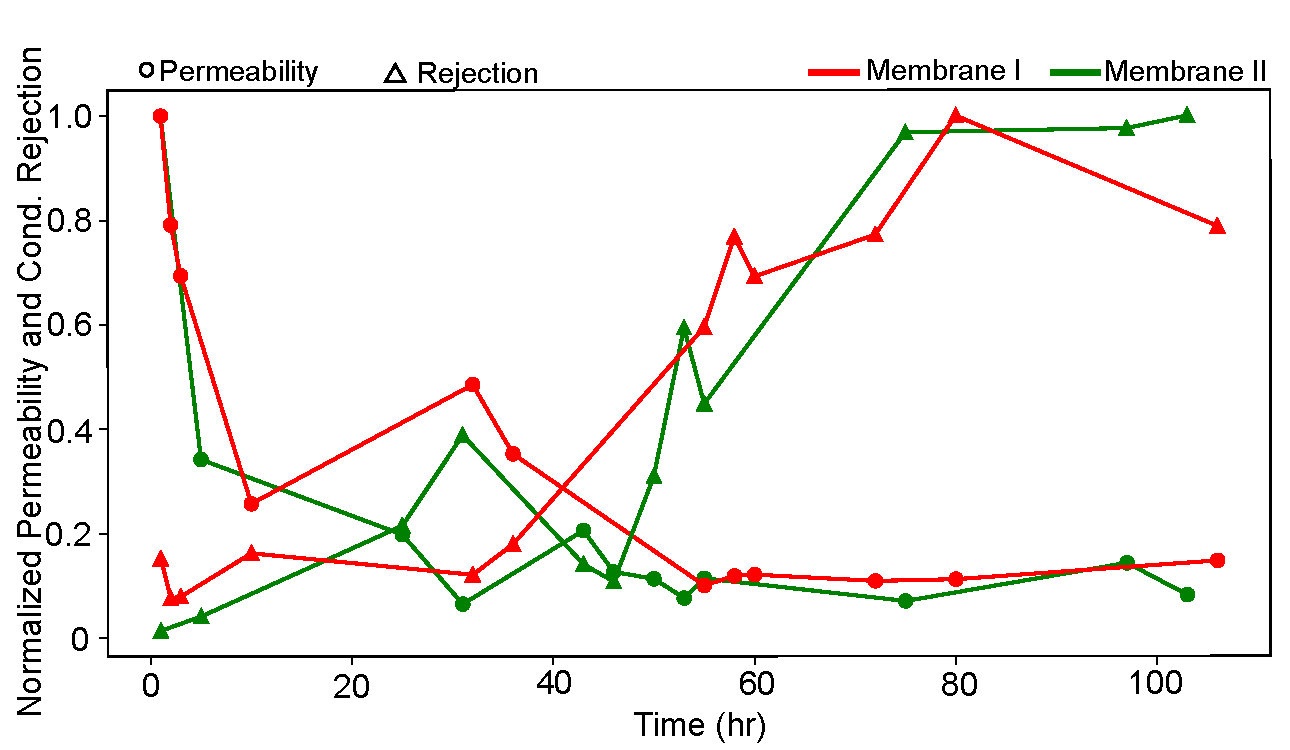
\includegraphics[width=5in]{paper5/Fig2.pdf}
  \caption{\textbf{FCM filtration ''representative'' measurements. Permeability (circles) and conductivity rejection (triangles) performance over time at 5 bar of applied pressure.} Colors represent different membranes tested (Membrane I in blue and Membrane II in green). The change over time is influenced by the compaction of the FCM hierarchical structure.}
  \label{Fig2_pap5}
\end{figure}


The steady-state permeability of the FCM was $1.3\pm0.6$ LMH-bar, which is in accordance with a previous study and is in the nanofiltration regime.\cite{amadei2017role} The triangles in Fig.~\ref{Fig2_pap5} represent the normalized conductivity rejection (R) of a solution containing monovalent (Na\textsuperscript{+}, Cl\textsuperscript{-}) and polyvalent ions (SO\textsubscript{4}\textsuperscript{2-}). As expected the conductivity rejection follows an inverse trend compared to the permeability with rejection increasing during GO selective layer compaction from $<10$\% to $\approx85$\%.
The specific ion rejection ($R_{ion}$) was then evaluated via ion chromatography of the feed and permeate (see Methods). The membranes display a moderate selectivity ($36\pm5$\%) for monovalent anions such as Cl\textsuperscript{-}. This is in agreement with other studies that highlighted the inefficacy of  GO membranes to sieve monovalent ions.\cite{chen2017molecular,baskoro2018graphene} However, we observe a greater selectivity ($86\pm4$\%)  for polyvalent ions such as sulfate. The diameter of the membrane pores ($d\textsubscript{pore}$) can be estimated using eqn~(\ref{eqn3_pap5}). For example, using the rejection values obtained for Cl\textsuperscript{-} and SO\textsubscript{4}\textsuperscript{2-} ($\approx36$\% and $\approx86$\%) and their corresponding hydrated diameters (0.66 and 0.76 nm), an average dpore of 1.83 and 1.05 nm, respectively, was estimated for the membranes. The discrepancy in the pore size dimension here is related to charge repulsion effects connected to the divalency of the sulfate anion, which increases rejection leading to smaller ''effective'' pore sizes estimated by eqn~(\ref{eqn3_pap5}). 
For GO membranes, the physical pore size or ''diameter'' is related to the interlayer distance (\textit{2d}) between GO flakes, which can be estimated from X-ray diffraction experiments. Previous X-ray diffraction studies indicate a \textit{2d} value around 0.8 nm for a dry GO membrane.\cite{amadei2017role,qi2017strict,hung2014cross} Under aqueous operation, the membrane will be hydrated and the GO laminate will undergo swelling characterized by a factor around 2, thus leading to a hydrated GO interlayer distance (\textit{2d}) between 1.5 and 2 nm.\cite{thebo2018highly,talyzin2014structure,yang2017ultrathin} This value range is in agreement with the dpore value estimated using chlorine rejection (\textit{i.e.}, 1.83 nm) and is also consistent with the results obtained in previous reports.\cite{abraham2017tunable}
\subsection{Fully Carbon Membrane Chemical Stability}
The FCM chemical stability was initially evaluated using the common oxidant sodium hypochlorite (NaClO).  Anions (Cl\textsuperscript{-}, SO\textsubscript{4}\textsuperscript{2-}) rejection before and after filtering 1000 ppm NaClO through the FCM for 9 hours at 5 bar is displayed in Fig.~\ref{Fig3_pap5}a. Chlorination did not have a significant effect on FCM anion rejection highlighting the FCM chemical resistance to oxidizing agents. The slight increase in observed FCM anion rejection suggests a decrease of the GO interlayer spacing as a result of NaClO addition, which increases the feed pH to 10 and reduces the ionic GO interlayer screening effect resulting in narrower GO channels/pore size.\cite{huang2013salt} This increase in anion rejection is also supported by the results obtained from CFP measurements, as shown in Fig.~\ref{Fig3_pap5}b. The chlorination process decreases the membranes wet flow by a factor of 5 at approximately 4 bar. The decrease and the absolute value of flow rate here cannot be directly compared to the valued obtained with the saline solutions as the CFP analysis is carried out with a lower surface tension wetting liquid (POREFIL\textsuperscript{\tiny\textregistered}, 16 dyne/cm) compared to that of water (72 dyne/cm). Moreover, the driving force behind the CFP is capillary, which is different as compared to the pressurized aqueous flow used in the cross-flow setup. In summary, the analyses completed here exemplify the FCM chemical stability and their resilience to oxidizing cleaning solutions since the extended application of concentrated NaClO did not have a significant effect on the FCM permeability and rejection.
\begin{figure}%[h!]
  \centering
  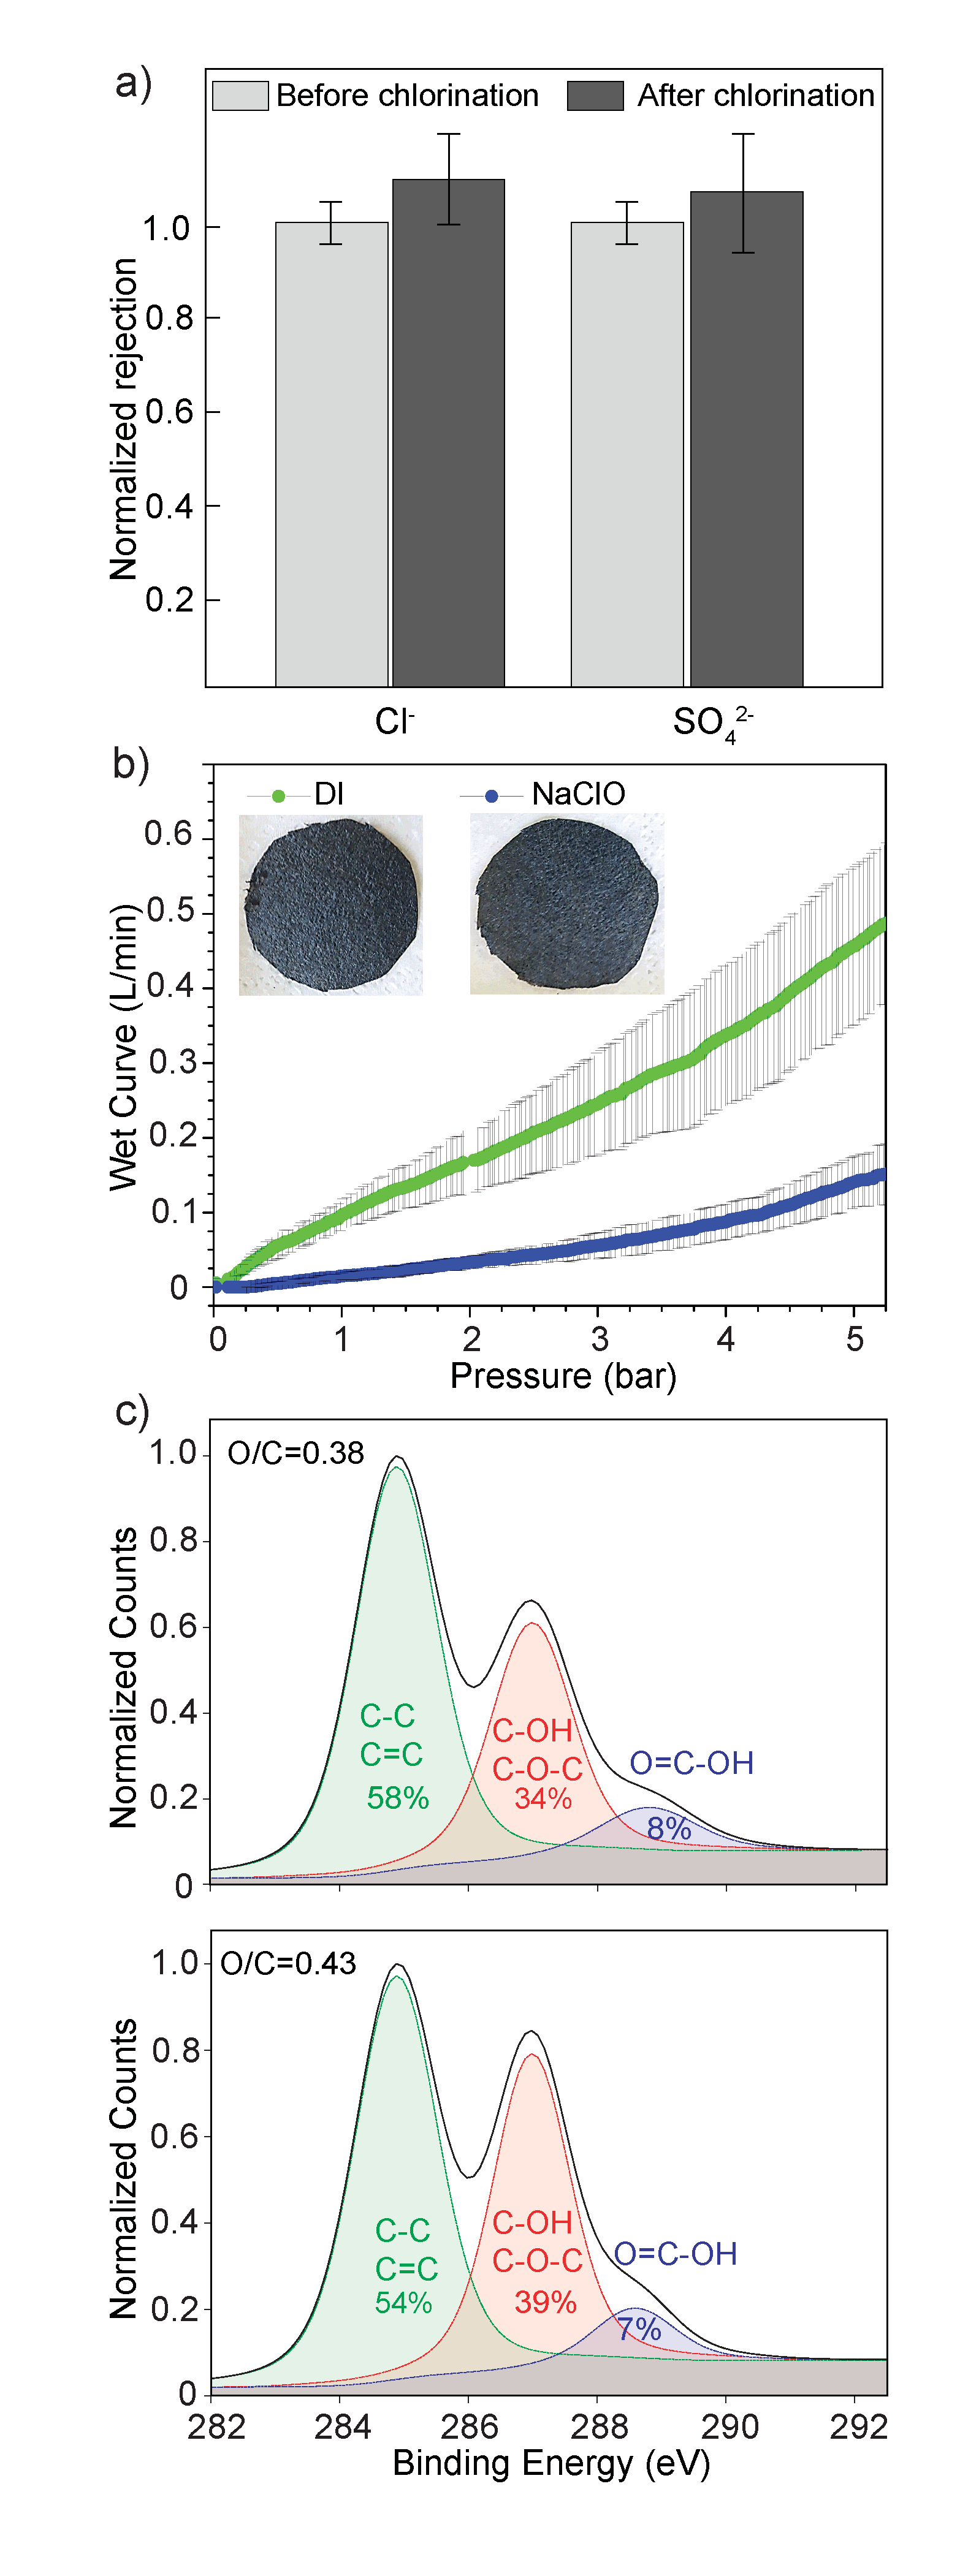
\includegraphics[width=3in]{paper5/Fig3.pdf}
  \caption{\textbf{FCM chemical stability.} \textbf{(a)} Normalized ions rejection before (light grey) and after (dark grey) chlorination. \textbf{(b)} CFP analysis of FCM after DI filtration (in green) and NaClO filtration (in blue). The figure includes photos of the FCMs used in the analysis. \textbf{(c)} C1s deconvolution spectra of the FCM before (top) and after (bottom) chlorination.}
  \label{Fig3_pap5}
\end{figure}
To further evaluate the FCM stability to oxidants, their surface chemistry was characterized via XPS as displayed in Fig.~\ref{Fig3_pap5}c. The untreated and chlorinated FCM are characterized by an XPS O/C ratio of 0.38 and 0.43, respectively, revealing minor surface oxidation post-chlorination. Even though the membranes were rinsed with copious DI water post-chlorination, the chlorinated FCM XPS is influenced by the presence of surface-associated ions, \textit{e.g.} 2\% Na in FCM atomic composition. The slightly increased O/C content of the chlorinated FCM can also be observed in the deconvolution of the C1s high resolution spectra, which is characterized by three peaks corresponding to: (i) single (C-C) and double (C=C) carbon bonds centered at 285 eV; (ii) epoxide (C-O-C) and hydroxide (C-OH) functional groups centered at 287 eV; and (iii) carboxylate (O=C-OH) functional groups centered at 289 eV. In particular, FCM chlorination results in a 4-5\% increase in the epoxide concentration, followed by the same magnitude decrease of the carbon sp\textsuperscript{2} signal centered at 285 eV.  Thermal annealing in an inert atmosphere would reduce the formed epoxides back to olefins returning the membranes to their original state.
FCM chemical stability was also challenged with common organic solvents such as acetone. The immersion of polyamide TFC membranes in acetone quickly and permanently degrades the membrane with the selective and ultrafiltration layers crumpling and detaching from the substrate. In stark contrast, the FCM are resistant to organic solvent degradation.  The FCM organic solvent stability can be also verified by examining SEM images presented in Fig.~\ref{figS7_AppD}, which reveals similar morphology (\textit{i.e.}, no visible damage) for FCM immersed in acetone compared to that of FCM immersed in water. For example, after acetone immersion, the GO and CNT layers still homogeneously cover the underlying CF paper, preserving its morphology as single carbon fibers are still recognizable. Stability to organic solvents may open new avenues for membrane cleaning \textit{e.g.} a CNT electrochemical filter poisoned with an insulating polymer coating could be regenerated using an organic solvent.\cite{gao2013electrocatalysis} Moreover, organic solvent resistance opens the FCM to a range of separation applications such as those in the petrochemical, food processing, and pharmaceutical industries, which commonly involve the use of aggressive aprotic solvents (\textit{e.g.}, acetone).\cite{chisca2015crosslinked}


\subsection{Fully Carbon Membrane Thermal Stability}
FCM thermal stability was initially evaluated during the fabrication process where the FCMs were reduced at 150 \textdegree C in a N\textsubrscript{2} atmosphere. No physical damage was observed to either the selective layer or the underlying substrate after this thermal annealing. The results of previous studies highlight the thermal stability of CNT and CF paper up to  $300-400$ \textdegree C in air;\cite{hordy2014high} and once reduced, GO tends to be stable under similar thermal conditions. More intense GO thermal treatment (\textit{e.g.}, T$>350$ \textdegree C) will lead to thermolysis of oxygen functionalities and possibly defect formation in the parent sp\textsuperscript{2} graphene sheet.\cite{bagri2010structural} To corroborate the FCM thermal stability,  the membranes were subjected to four sequential thermal annealing cycles of 15 min at 150 \textdegree C in an oxidizing environment (\textit{i.e.}, ambient air). Afterwards, the XPS C1s peak profiles of the FCM (see Fig.~\ref{Fig4_pap5} and Table~\ref{tblS1_AppD}in the Appendix D) were used to evaluate the effect of the annealing cycles on the FCM surface chemistry. The sp\textsuperscript{2} peak (C-C; C=C) is constant at $\approx65$\% before and after every annealing cycle highlighting the FCM thermal stability. A TGA (Fig.~\ref{figS8_AppD} in the Appendix D) indicates that the FCM is stable until 350 \textdegree C with less than 0.1\% loss in mass; at this temperature, the $\Delta$m/$\Delta$T begins to increase signaling the onset of FCM thermal decomposition. For comparison, a traditional polyamide TFC is observed to lose 70\% of its mass by 500 \textdegree C, whereas the loss is $<1$\% for an FCM. The FCM thermal stability can be utilized for membrane regeneration similar to ceramic membranes, in which the regeneration temperature ($>200$ \textdegree C) depends on the adsorbed/deposited species.\cite{liu2018functionalized} The superior FCM thermal stability compared to traditional polymeric membranes will increase potential for a broader range of industrial applications such as the treatment of cooling/boiler water in thermoelectric generation plants or oil/water separations in petroleum processing plants. 

\begin{figure}[h!]
  \centering
  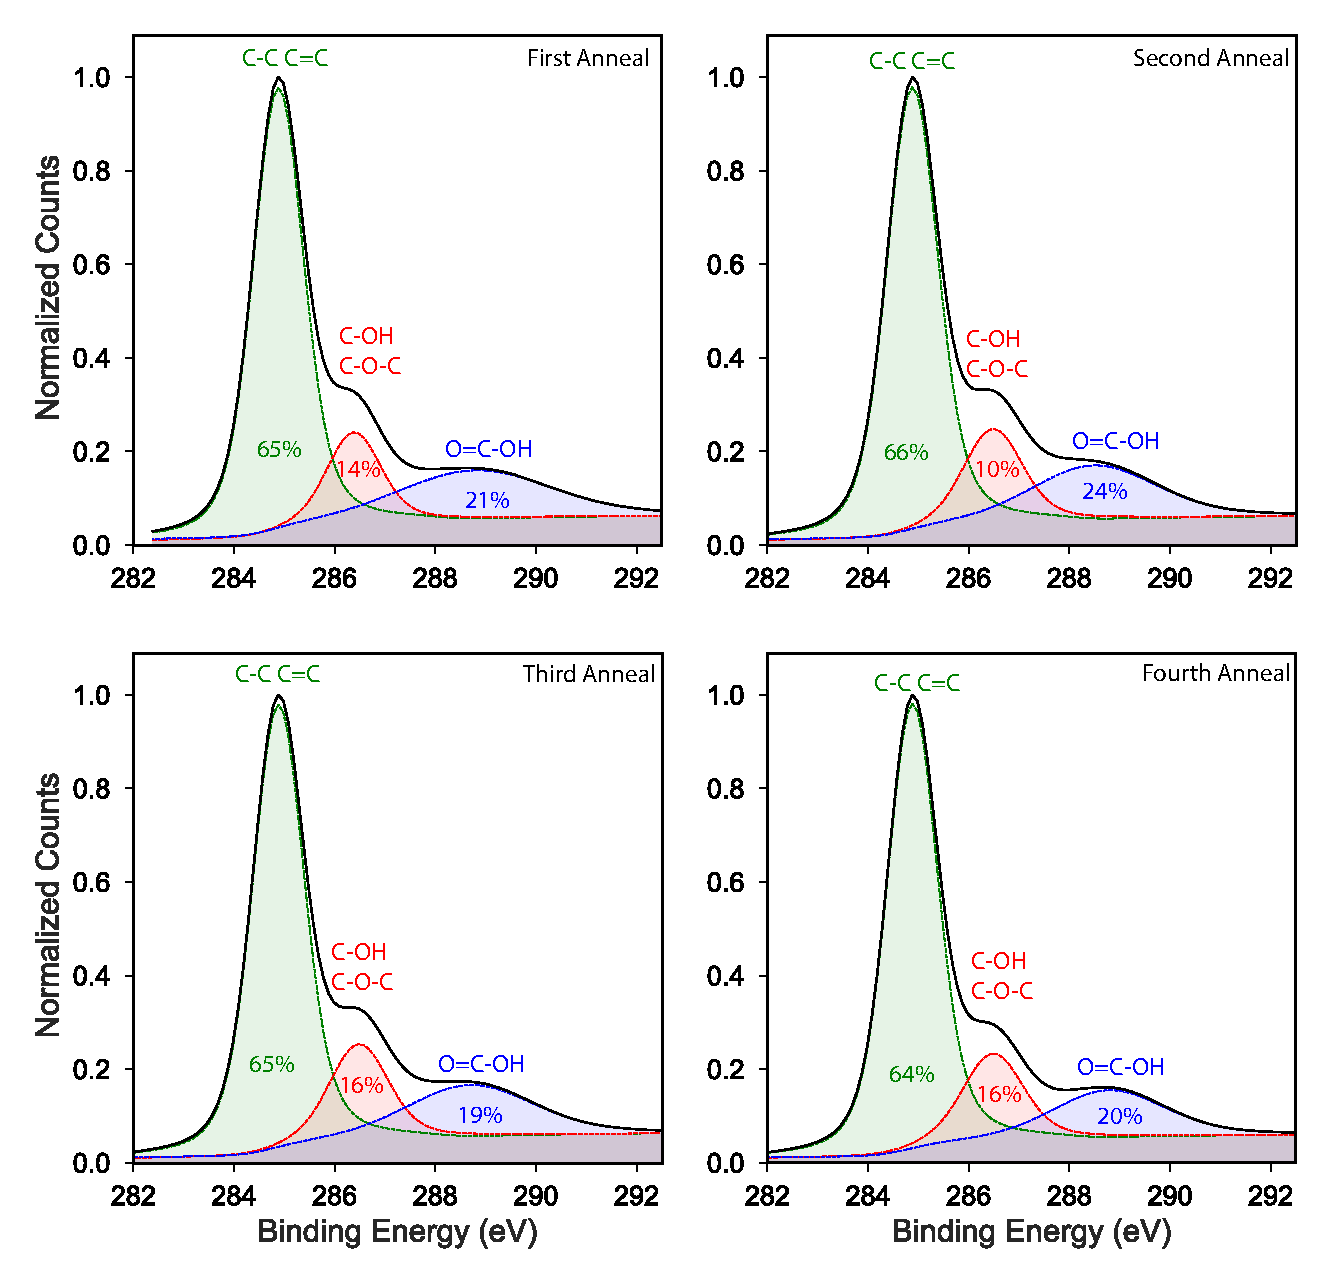
\includegraphics[width=5in]{paper5/Fig4.pdf}
  \caption{\textbf{FCM thermal stability.} C1s deconvolution spectra of the FCM subjected to four annealing cycles of 15 min at 150 \textdegree C in an oxidizing environment (\textit{i.e}, ambient air).}
  \label{Fig4_pap5}
\end{figure}



\subsection{Non-linear and Reversible Permeability Pressure-dependence}
Here, the FCM pressure-dependent permeability post-compaction was investigated as displayed in Fig.~\ref{Fig5_pap5}.  Of note is that when the applied pressure is increased from 4.5 to 7.5 bar (1.67-fold) the normalized permeability (in red) increases from 0.4 to 0.9 (2.25-fold) (see Fig.~\ref{Fig1_pap5}), which is at odds with Darcy's Law that predicts a pressure-independent permeability. This behavior has been previously reported both experimentally and through molecular dynamic simulations for carbon nanostructures \cite{liu2018functionalized, nicolai2014tunable} and it differs from polymeric membranes behavior, where the pressure-normalized flux (\textit{i.e.}, LMH-bar) is invariant of the applied pressure. The increase in permeability with increasing pressure is corroborated by a concomitant decrease in ion rejection of around 1.6-fold (in green). The decrease in the rejection at higher pressures may be related to the energy barrier required to dehydrate ions since similar barrier is also present in the disruption of the hydrogen bond network for water entering in the GO nanochannels from the bulk. However, the latter energy is significantly lower than the necessary dehydration of ions ($\approx6$ kJ/mol versus 102-103 kJ/mol); in other words, the low pressure increase ($\approx3$ bar) provides enough energy to break the hydrogen bonding network, but is not sufficient for the dehydration of the ions.\cite{thomas2016computational} Thus, pressure-induced ion dehydration is likely not active here.
Thus at first glance, the decrease in the rejection could also be attributed to pressure-induced membrane damage. However, once the pressure is reduced back to 4.5 bar the FCM permeability and rejection reversibly return to their original state and this phenomenon was reproduced with a number of FCM samples. The reversibility of FCM performance with pressure could be a noteworthy addition to the recent developments in the field of active membranes. In particular, there is a continuous effort to develop smart membranes that are active and/or reactive in response to external stimuli. A recent study demonstrated that GO membrane performance can be altered by an externally applied unidirectional force.\cite{li2018controlling} GO studies have also used other externally applied stimuli such as voltage, which ionizes water molecules inside the GO channel leading to a blockage of water transport.\cite{zhou2018electrically} Similarly, studies have attempted to modify the structure of the GO nanochannel by altering the pH of the feed, inducing pH-dependent membrane performance phenomena.\cite{oh2017understanding} Thus, the ability of the GO nanostructure to adapt to multiple external stimuli makes it an ideal candidate for the fabrication of structurally-active membranes with reversible behavior.
\begin{figure}[h!]
  \centering
  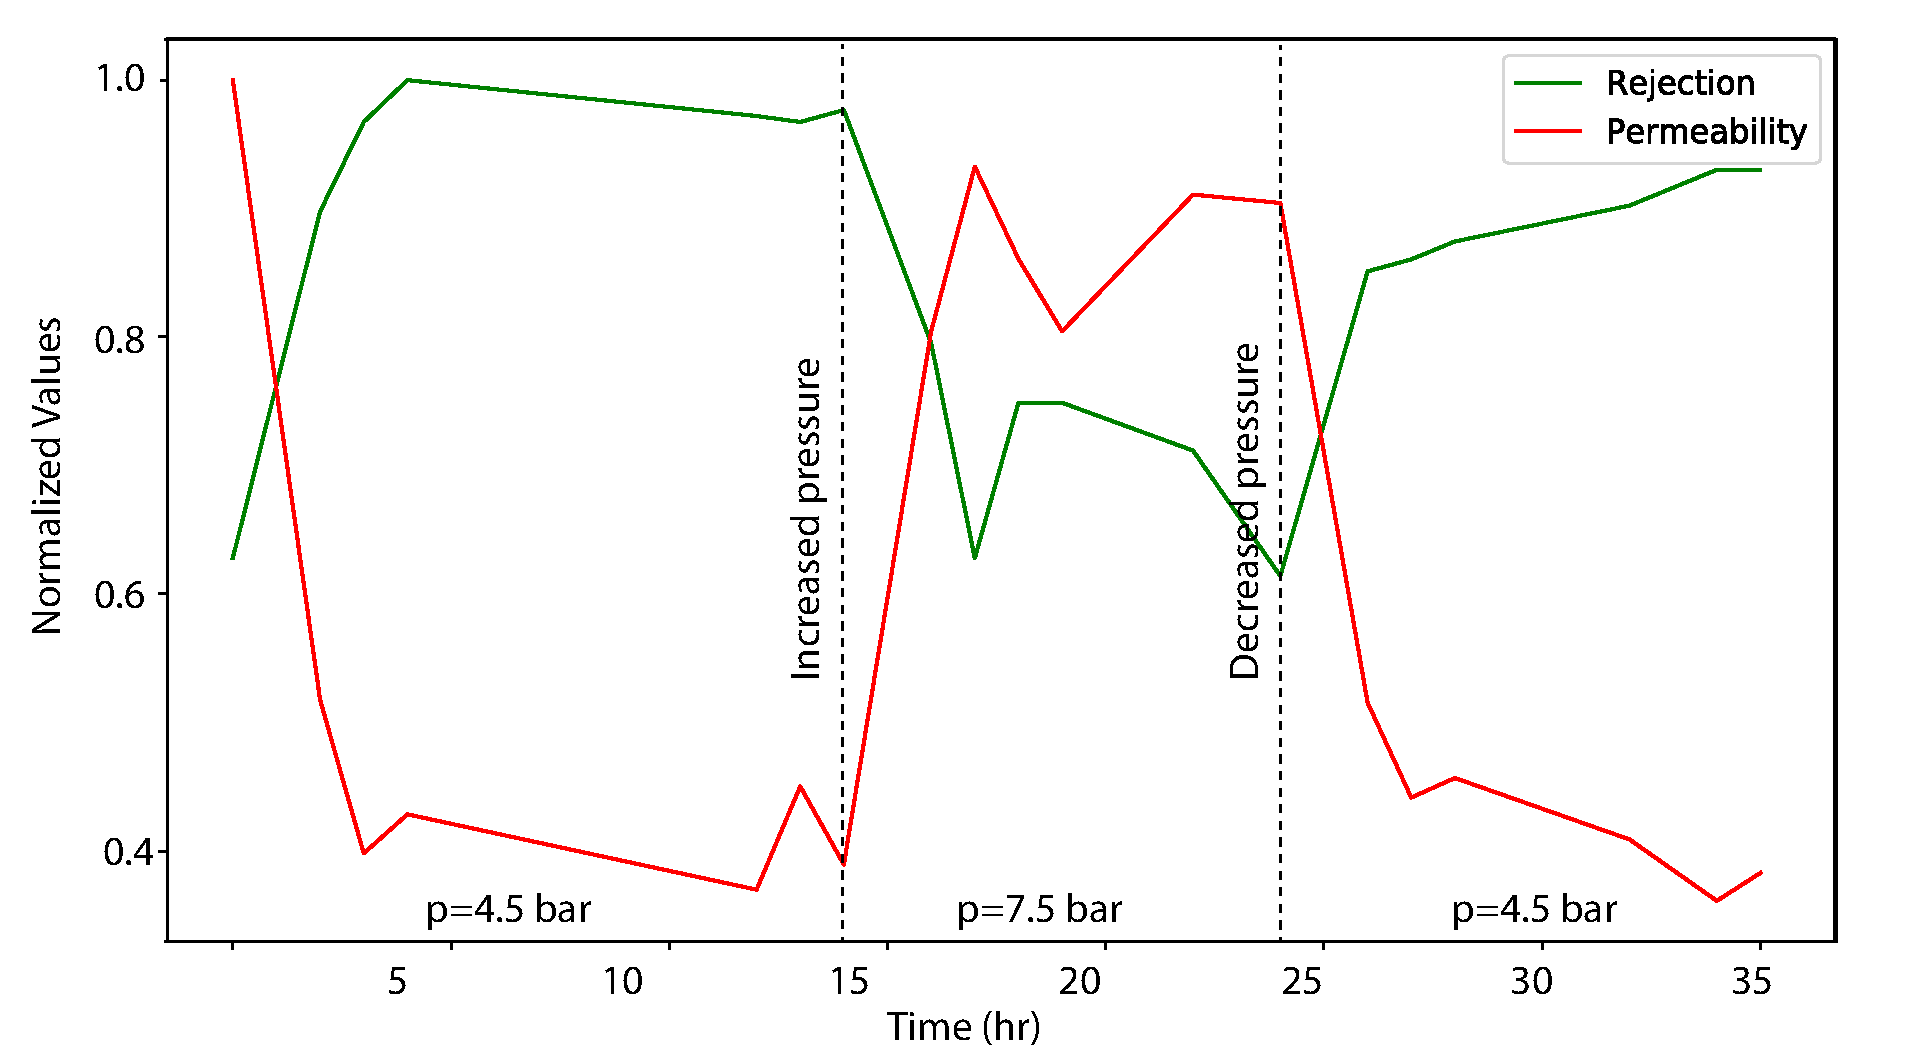
\includegraphics[width=5in]{paper5/Fig5.pdf}
  \caption{\textbf{FCM reversible behavior.} Permeability (in red) and rejection (in green) performance of a FCM over time under different pressures applied. The dashed line indicates the times when the pressure was changed.}
  \label{Fig5_pap5}
\end{figure}


\section{Conclusions}
This investigation highlights the possibility of creating a new class of fully carbon membranes that possess the combined advantages of typically disparate polymeric and ceramic membranes, thus completing the Hegelian triad. The unique FCM characteristics are a result of the layer-by-layer nano-manipulation of the elemental carbon architectures embedded in its hierarchical structure.  The FCM operates in the nanofiltration regime similar to polymeric and, concurrently display the chemical and thermal stability typical of ceramic membranes. Specifically, FCM have a nanoscale pore size ($<2$ nm), which effectively reject polyvalent ions, and are also resistant to chlorine oxidants, high pH, organic solvents, and elevated temperatures ($>150$ \textdegree C). The investigation also displayed the ability to use externally applied pressure as a potential stimulus to control performance in situ, highlighting the structurally-active and reversible behavior of the FCM. Through the development of an FCM we are hoping to spark a new direction of research in membrane materials displaying polymer-ceramic hybrid properties, cultivating new material ideas, promoting membrane progress, supporting continued AWWT efforts, and thus ultimately contributing to the increase of global water resources.
